\documentclass[10pt]{beamer}
\usetheme{metropolis}
\usecolortheme{default}
\usepackage{booktabs}
\usepackage{amsmath}
\usepackage{graphicx}
\usepackage{tikz}
\usepackage{pgfplots}
\pgfplotsset{compat=1.17}
\usetikzlibrary{arrows.meta, positioning, calc, shapes, fit, backgrounds, patterns}
\definecolor{myTeal}{HTML}{23373b}
\definecolor{myOrange}{HTML}{EB811B}
\setbeamercolor{alerted text}{fg=myOrange}

\title{Interest Groups, Rent-Seeking and Lobbying}
\subtitle{ECO1028 -- Politics Without Romance}
\author{Beatriz Gietner\\
\texttt{beatriz.gietner@dcu.ie}}
\date{\today}

\begin{document}

\maketitle

\begin{frame}{Outline}
\tableofcontents
\end{frame}

\section{Why Do Small Groups Win?}

\begin{frame}{Before We Begin: A Diagnostic Question}
\textbf{Imagine the government is considering a new policy:}

\begin{itemize}
\item A tariff on imported steel that gives \alert{\euro 10 million} in extra profit to 5 domestic steel firms
\item The cost: every citizen pays roughly \alert{\euro 2 more} per year on goods containing steel
\end{itemize}

\vspace{0.2cm}
\textbf{Quick poll:}
\begin{itemize}
\item A) The tariff will \emph{pass} - the steel firms will lobby for it
\item B) The tariff will \emph{fail} - citizens will oppose it
\item C) It depends on the political system
\end{itemize}

\vspace{0.2cm}
\alert{Follow-up:} Why would 5 million people each losing \euro 2 fail to block 5 firms each gaining \euro 2 million?
\end{frame}


\begin{frame}{The Central Puzzle of This Lecture}
\textbf{Three related questions:}

\begin{itemize}
\item \textbf{Olson:} Why do small groups organise while large groups do not?
\item \textbf{Tullock:} What resources are wasted in the fight for special privileges?
\item \textbf{Stigler:} Who actually benefits from government regulation?
\end{itemize}

\vspace{0.2cm}
\alert{Common thread:} the interaction between group size, incentives, and political outcomes systematically favours concentrated interests over the general public.

\vspace{0.2cm}
\textbf{Public Choice perspective:}
\begin{itemize}
\item Regulation is not handed down by benevolent planners
\item It is shaped by the same self-interested actors we study in markets
\end{itemize}
\end{frame}


\begin{frame}{Key Definitions (for today)}
\small
\begin{itemize}
\item \textbf{Interest group:} an organised body that seeks to influence government policy on behalf of its members.
\item \textbf{Collective action problem:} when individually rational behaviour (free-riding) leads to a collectively suboptimal outcome (Olson's).
\item \textbf{Free-riding:} benefiting from a group good without contributing to its provision.
\item \textbf{Selective incentive:} a benefit available only to those who participate in collective action (Olson's).
\item \textbf{Rent:} income above what a resource could earn in its next best use; often created by government restriction.
\item \textbf{Rent-seeking:} spending real resources to acquire, maintain, or protect a rent (Tullock's).
\item \textbf{Regulatory capture:} when a regulatory agency acts primarily in the interest of the industry it is supposed to regulate (Stigler's).
\item \textbf{Concentrated benefits / dispersed costs:} a policy whose gains accrue to a few while its costs are spread across many.
\end{itemize}
\end{frame}


\begin{frame}{What We Will Learn}
\textbf{By the end of this lecture, you should understand:}

\begin{itemize}
\item Why \alert{small groups} organise more easily than large ones (Olson)
\item Why the resources spent competing for rents can be as wasteful as the rents themselves (Tullock)
\item Why regulation often serves \alert{producers}, not consumers (Stigler)
\item How these three ideas connect into a coherent Public Choice view of interest-group politics
\end{itemize}

\vspace{0.2cm}
\textbf{Core readings:}
\begin{itemize}
\item Olson (1965), \emph{The Logic of Collective Action} (excerpts)
\item Tullock (1967), "The Welfare Costs of Tariffs, Monopolies, and Theft"
\item Stigler (1971), "The Theory of Economic Regulation"
\end{itemize}
\end{frame}

\section{Olson: The Logic of Collective Action}

\begin{frame}{The Traditional View (Pre-Olson)}
\textbf{Before Olson, political scientists generally assumed:}

\begin{itemize}
\item Groups with shared interests naturally organise to pursue them
\item Larger groups are more powerful because they have more members
\item The political system reflects the "balance of group pressures"
\end{itemize}

\vspace{0.2cm}
\alert{Olson's challenge:} this reasoning ignores the \emph{internal} economics of the group.

\vspace{0.2cm}
If a tariff benefits all steel producers, each firm benefits whether or not it contributes to the lobbying effort.
The tariff is a \textbf{public good} within the group - and public goods are underprovided
\end{frame}


\begin{frame}{Why Groups Fail: The Free-Rider Problem}
\textbf{Olson's core insight:}

A shared interest is \emph{necessary but not sufficient} for collective action.
The obstacle is the same one that makes public goods hard to provide voluntarily.

\vspace{0.2cm}
\textbf{Consider a group of $N$ firms that share an interest:}
\begin{itemize}
\item The benefit of successful lobbying is shared by all $N$ firms
\item But the cost of lobbying falls only on those who contribute
\item Each firm has an incentive to let others bear the cost
\end{itemize}

\vspace{0.2cm}
\alert{Result:} the larger the group, the stronger the temptation to free-ride, and the less likely the group is to act collectively.
\end{frame}


\begin{frame}{Why Is Group Size Important}
\textbf{Olson identifies three mechanisms that make small groups more effective:}

\vspace{0.1cm}
\begin{enumerate}
\item \textbf{Per-capita stakes are higher.}
If a \euro 10m rent is split among 5 firms, each stands to gain \euro 2m.
If a \euro 10m cost is spread over 5 million citizens, each loses \euro 2.
The firms have far stronger incentives to act.

\vspace{0.1cm}
\item \textbf{Defection is visible.}
In a group of 5, everyone knows who is contributing and who is not.
In a group of 5 million, no individual's absence is noticed.

\vspace{0.1cm}
\item \textbf{Coordination costs are lower.}
Agreeing on strategy, dividing costs, and monitoring compliance is easy with 5 members, prohibitively difficult with 5 million.
\end{enumerate}
\end{frame}

\begin{frame}{Small vs Large Groups}
\begin{center}
\includegraphics[width=0.9\linewidth]{img1.png}
\end{center}
“The larger the group, the less it will further its common interests.”
- Olson (1965)
\end{frame}


\begin{frame}{How Large Groups \emph{Can} Organise: Selective Incentives}
\textbf{If large groups never organised, we would never see trade unions, consumer movements, or environmental lobbies.}

\vspace{0.1cm}
Olson argues large groups succeed only when they offer \alert{selective incentives} - private benefits available exclusively to contributors:

\vspace{0.1cm}
\begin{itemize}
\item \textbf{Material:} insurance, legal advice, discounts
\begin{itemize}
\item[\footnotesize$\triangleright$] \footnotesize Trade unions: legal representation, workplace protection
\end{itemize}
\item \textbf{Solidary:} social belonging, status, identity
\begin{itemize}
\item[\footnotesize$\triangleright$] \footnotesize Professional associations: networking, prestige
\end{itemize}
\item \textbf{Coercive:} mandatory membership, social pressure
\begin{itemize}
\item[\footnotesize$\triangleright$] \footnotesize Closed-shop agreements, professional licensing requirements
\end{itemize}
\end{itemize}

\vspace{0.1cm}
\alert{Key implication:} the political activity of large groups is often a \emph{by-product} of organisations that exist for other reasons.
\end{frame}


\begin{frame}{Discussion: Can You Identify the Selective Incentive?}
\textbf{For each group, what keeps members from free-riding?}

\vspace{0.1cm}
\begin{enumerate}
\item The Irish Farmers' Association (IFA)
\item A neighbourhood residents' association opposing a local development
\item The Irish Medical Organisation (IMO)
\item An online petition to reduce university fees
\end{enumerate}

\vspace{0.2cm}
\alert{Think about:}
\begin{itemize}
\item How large is the group?
\item Is the benefit excludable?
\item What happens if you do not contribute?
\end{itemize}
\end{frame}


\begin{frame}{Olson's Legacy: What Carries Forward}
\textbf{Three takeaways that feed into the rest of today's lecture:}

\vspace{0.1cm}
\begin{enumerate}
\item \textbf{Asymmetry is the default.}
Policies with concentrated benefits and dispersed costs will tend to be adopted, because the beneficiaries organise and the losers do not.

\vspace{0.1cm}
\item \textbf{Political outcomes $\neq$ efficiency outcomes.}
The political "market" is biased toward groups that can overcome collective action problems, not toward the policies with the highest social welfare.

\vspace{0.1cm}
\item \textbf{The missing counter-lobby.}
When you see a policy that benefits a small group at the expense of many, the puzzle is not why the group lobbied for it - it is why no one lobbied against it.
\end{enumerate}

\vspace{0.1cm}
\alert{Next question:} What is the \emph{social cost} of all this lobbying activity?  $\rightarrow$ Tullock.
\end{frame}


\begin{frame}{Olson's Dynamic Extension: Institutional Sclerosis}
\textbf{In \emph{The Rise and Decline of Nations} (1982), Olson extends the argument to economic growth:}

\vspace{0.1cm}
\begin{itemize}
\item Stable democracies \alert{accumulate} interest groups over time
\item Each group extracts a small rent; the aggregate drag becomes significant
\item These "distributional coalitions" resist reform, slow resource reallocation, and raise transaction costs
\end{itemize}

\vspace{0.1cm}
\textbf{The striking prediction:}
Countries whose interest-group networks were \emph{destroyed} - by war, revolution, or regime change - should grow faster afterwards.

\vspace{0.1cm}
\alert{Evidence:} post-war Germany and Japan grew faster than Britain, whose interest-group structures survived intact.
Ireland's post-1987 recovery is sometimes read through the same lens: crisis enabled reforms that entrenched coalitions had blocked.
\end{frame}

\section{Tullock: The Welfare Cost of Rent-Seeking}

\begin{frame}{The Standard Welfare Analysis: What's Missing?}
\textbf{Before Tullock, the welfare cost of a monopoly or tariff was measured as:}

\vspace{0.1cm}
\begin{itemize}
\item The \textbf{deadweight loss} triangle - the transactions that no longer occur because of the distorted price
\item The \textbf{transfer} from consumers to producers was treated as a pure redistribution, not a social cost
\end{itemize}

\vspace{0.2cm}
\alert{Tullock's question (1967):}
If a tariff creates \euro 10m in rents for domestic producers, how much will they spend trying to \emph{obtain} that tariff?

\vspace{0.1cm}
If the answer is "up to \euro 10m," then the transfer rectangle is not merely redistributive - it represents real resources consumed in the contest for political favours.
\end{frame}



\begin{frame}{Why the Transfer Becomes a Social Cost}
\textbf{Tullock's reasoning:}

\begin{enumerate}
\item A tariff or monopoly licence creates a \alert{rent} - income above competitive returns.
\item Rational agents will invest resources to capture that rent: lobbying, lawyers, campaign contributions, public relations.
\item These expenditures are \textbf{socially wasteful}: they do not produce goods or services; they only determine who gets the transfer.
\item In the limit, competing rent-seekers may dissipate the \emph{entire value of the rent} in contest expenditures.
\end{enumerate}

\vspace{0.1cm}
\alert{Analogy:} 
Imagine 10 people each spending \euro 90,000 in legal fees to win a \euro 100,000 inheritance.
The winner gains \euro 10,000 net; society loses \euro 900,000 in wasted legal resources.
\end{frame}

\begin{frame}{How Large Are Rent-Seeking Costs?}
\textbf{Tullock's original examples:}

\begin{itemize}
\item \textbf{Tariffs:} firms spend on lobbying, trade associations, and legal challenges
\item \textbf{Monopoly licences:} applicants invest in political relationships and compliance theatre
\item \textbf{Theft:} both thieves and victims invest in the contest (locks, alarms, security vs tools and risk)
\end{itemize}

\vspace{0.1cm}
\textbf{The empirical implication:}
\begin{itemize}
\item Harberger (1954) estimated US monopoly welfare losses at $\approx$ 0.1\% of GDP
\item If rent-seeking costs are of the same order as the rents themselves, the true social cost could be \alert{10--100 times larger}
\end{itemize}

\vspace{0.1cm}
\footnotesize
\alert{This is why "rent-seeking" became one of the most cited concepts in political economy.}
\end{frame}


\begin{frame}{Tullock's Provocation: Tariffs, Monopoly, and Theft}
\textbf{The most striking move in Tullock's 1967 paper is treating tariffs, monopoly, and theft as analytically identical.}

\vspace{0.1cm}
In each case, resources flow into a \alert{distributional contest} rather than into production:

\vspace{0.1cm}
\begin{itemize}
\item \textbf{Theft:} a burglar invests in tools and risk; a homeowner invests in locks and alarms.
Neither investment produces anything - both exist solely because of the contest.

\item \textbf{Monopoly:} a firm invests in lobbying and political connections to obtain or defend a licence.

\item \textbf{Tariffs:} domestic producers invest in trade-association campaigns and public relations.
\end{itemize}

\vspace{0.1cm}
\alert{Tullock's point:} from a welfare perspective, the resources consumed in each contest are equally wasteful.
The legal status of the activity is irrelevant to the economic analysis - a claim that tends to provoke strong reactions, especially from law students.
\end{frame}


\begin{frame}{From Tullock to Stigler: The Bridge}
\textbf{Tullock showed us \emph{how much} is wasted.}

\vspace{0.1cm}
\textbf{But who wins these contests?}

\begin{itemize}
\item Olson tells us \emph{small, concentrated groups} organise more easily
\item Tullock tells us those groups will spend heavily to capture rents
\item But where exactly do they seek these rents?
\end{itemize}

\vspace{0.2cm}
\alert{Stigler's answer:} the regulatory process itself.

\vspace{0.1cm}
Government regulation is not imposed on industries from outside.
Industries actively \emph{seek} regulation as a tool for restricting competition, raising barriers to entry, and protecting profits.
\end{frame}


\section{Stigler: The Theory of Economic Regulation}

\begin{frame}{The Puzzle Stigler Starts With}
\textbf{Standard public-interest theory of regulation:}
\begin{itemize}
\item Regulation exists to correct market failures
\item It protects consumers from monopoly power, externalities, and asymmetric information
\end{itemize}

\vspace{0.2cm}
\alert{But Stigler observes patterns that this theory cannot explain:}

\begin{itemize}
\item Trucking regulation restricted entry and \emph{raised} freight rates
\item Occupational licensing limited supply and \emph{raised} prices for consumers
\item Airlines, taxis, and banking all experienced \emph{higher} prices under regulation
\item Regulated industries often \emph{lobbied to keep} their regulations
\end{itemize}

\vspace{0.1cm}
\alert{If regulation protects consumers, why do producers fight to preserve it?}
\end{frame}


\begin{frame}{Stigler's Central Thesis}


\textbf{"As a rule, regulation is acquired by the industry and is designed and operated primarily for its benefit." — Stigler (1971)}

\vspace{0.1cm}
{\footnotesize - George Stigler, "The Theory of Economic Regulation" (1971)}

\vspace{0.2cm}
Stigler reframes regulation as a \alert{market}: industries demand favourable regulation, and politicians supply it in exchange for political support.

\vspace{0.1cm}
\textbf{Do not think of this as corruption in the traditional sense.}
It is the normal, predictable outcome of rational agents operating within political institutions - exactly the kind of analysis Public Choice applies.
\end{frame}


\begin{frame}{What Do Industries Want from the State?}
\textbf{Stigler identifies four benefits industries seek through regulation:}

\vspace{0.1cm}
\begin{enumerate}
\item \textbf{Direct subsidies}
\begin{itemize}
\item[\footnotesize$\triangleright$] \footnotesize Cash transfers, tax breaks, grants
\end{itemize}

\item \textbf{Control over entry of new competitors}
\begin{itemize}
\item[\footnotesize$\triangleright$] \footnotesize Licensing, permits, qualifications - the most powerful tool
\end{itemize}

\item \textbf{Policies affecting substitutes and complements}
\begin{itemize}
\item[\footnotesize$\triangleright$] \footnotesize Tariffs on imports, restrictions on adjacent industries
\end{itemize}

\item \textbf{Price-fixing}
\begin{itemize}
\item[\footnotesize$\triangleright$] \footnotesize Minimum prices, rate-of-return regulation
\end{itemize}
\end{enumerate}

\vspace{0.1cm}
\alert{Why is entry control preferred over cash subsidies?}
Because restricting entry prevents new firms from eroding the rent through competition.
A cash subsidy attracts entrants; a licence keeps them out.
\end{frame}


\begin{frame}{The Political Market for Regulation}
\centering
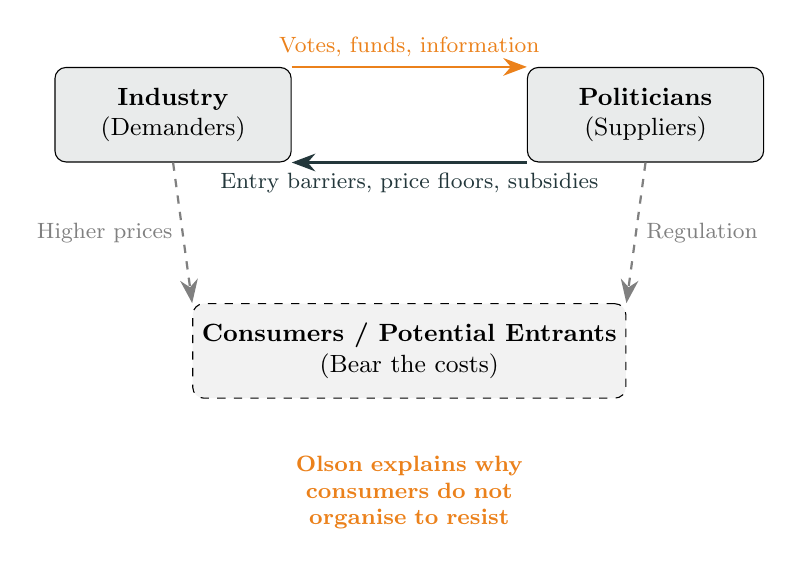
\begin{tikzpicture}[
node distance=2.5cm,
box/.style={draw, rounded corners, minimum width=3cm, minimum height=1.2cm, align=center, font=\small},
arrow/.style={-{Stealth[length=3mm]}, thick}
]

\node[box, fill=myTeal!10] (industry) at (-3,0) {\textbf{Industry}\\(Demanders)};
\node[box, fill=myTeal!10] (politicians) at (3,0) {\textbf{Politicians}\\(Suppliers)};

\draw[arrow, myOrange] (industry.north east) -- node[above, font=\footnotesize, sloped] {Votes, funds, information} (politicians.north west);
\draw[arrow, myTeal] (politicians.south west) -- node[below, font=\footnotesize, sloped] {Entry barriers, price floors, subsidies} (industry.south east);

\node[box, fill=gray!10, dashed] (consumers) at (0,-3) {\textbf{Consumers / Potential Entrants}\\(Bear the costs)};
\draw[arrow, gray, dashed] (politicians.south) -- node[right, font=\footnotesize] {Regulation} (consumers.north east);
\draw[arrow, gray, dashed] (industry.south) -- node[left, font=\footnotesize] {Higher prices} (consumers.north west);

\node[font=\footnotesize, text=myOrange, text width=4.5cm, align=center] at (0,-4.8) {\textbf{Olson explains why consumers do not organise to resist}};
\end{tikzpicture}
\\
\vspace{0.1cm}
“The state - the machinery and power of the state - is a potential resource or threat to every industry in the society.”
— Stigler (1971)
\end{frame}


\begin{frame}[allowframebreaks]{Is the “Political Market” Framing Correct?}
\small

\textbf{Core structure (Public Choice view):}
\begin{itemize}
\item \textbf{Industry} demands regulation (rents)
\item \textbf{Politicians} supply policy in exchange for political support
\item \textbf{Exchange:}
\begin{itemize}
\item Industry $\rightarrow$ votes, funds, information
\item Politicians $\rightarrow$ entry barriers, price floors, subsidies
\end{itemize}
\item \textbf{Consumers} bear diffuse costs
\end{itemize}


\textbf{Foundations:}
\begin{itemize}
\item \textbf{Olson (1965):} large groups do not organise (free-riding)
\item \textbf{Stigler (1971):} regulation as capture
\item \textbf{Peltzman (1976):} politicians maximise political support
\item \textbf{Becker (1983):} equilibrium of competing pressure groups
\end{itemize}


\textbf{Refinement:}
\begin{itemize}
\item Regulation is the \emph{channel} through which costs reach consumers
\item Politicians maximise political support; regulation is an instrument
\item Outcome reflects the relative political power of organised groups
\end{itemize}

\end{frame}


\begin{frame}{Why Small Industries Capture Regulation}
\textbf{Stigler connects directly to Olson:}

\vspace{0.1cm}
The "price" an industry pays for regulation comes in two currencies:
\begin{itemize}
\item \textbf{Votes:} the industry and its employees vote as a bloc
\item \textbf{Resources:} campaign contributions, information provision, revolving-door employment
\end{itemize}

\vspace{0.1cm}
\textbf{Compact industries are more effective because:}
\begin{itemize}
\item They can \alert{monitor} politicians' compliance with implicit deals
\item They face lower \alert{coordination costs} in agreeing on what to demand
\item They can \alert{punish} defectors more credibly (withdraw support)
\end{itemize}

\vspace{0.1cm}
\alert{Stigler's prediction:}
Regulation will tend to benefit industries that are \emph{small enough to organise} but \emph{large enough to offer meaningful political resources}.
\end{frame}


\begin{frame}{The Information Channel: Why Regulators Depend on Industry}
\textbf{Capture is not always about money or votes.}

\vspace{0.15cm}
Regulators face an \alert{information asymmetry}: the industry they regulate understands its own technology, costs, and risks far better than any government agency.

\begin{itemize}
\item A TD deciding on pharmaceutical regulation needs technical expertise
\item The industry itself is the cheapest and most available supplier
\item Over time, regulators come to rely on the regulated for the knowledge needed to regulate
\end{itemize}

\vspace{0.15cm}
\textbf{This creates a subtler form of capture:}
Not bribery, not even conscious bias - but a structural dependence that tilts the information environment in the industry's favour.

\vspace{0.15cm}
\footnotesize
\alert{Carpenter (2010):} the FDA illustrates how expertise-dependence can coexist with genuine regulatory effort.
\end{frame}


\begin{frame}{The Revolving Door}
\textbf{One of the most visible mechanisms of information capture:}

\vspace{0.1cm}
\begin{itemize}
\item \textbf{Industry $\rightarrow$ regulator:} former industry employees bring expertise but also sympathies and networks
\item \textbf{Regulator $\rightarrow$ industry:} the prospect of lucrative post-government employment creates incentives not to antagonise future employers
\end{itemize}

\vspace{0.1cm}
\textbf{Why does the revolving door exist?}
Partly because regulators \emph{need} people who understand the industry.
The same information asymmetry that enables capture also makes the revolving door functionally necessary.

\vspace{0.1cm}
\alert{Irish examples:}
\begin{itemize}
\item Financial regulators moving to banking and consultancy after 2008
\item Energy regulators (CRU) and the energy industry
\item Planning officials and property development
\end{itemize}
\end{frame}


\begin{frame}{Case Study: Occupational Licensing}
\textbf{A textbook example of regulatory capture in action.}

\vspace{0.1cm}
\textbf{The pattern:}
\begin{enumerate}
\item A profession argues licensing is needed to protect consumers from incompetent practitioners
\item The licensing board is staffed by members of the profession itself
\item Entry requirements are set high enough to restrict supply
\item Prices rise; existing practitioners earn rents
\item Consumers have no organised voice in the process
\end{enumerate}

\vspace{0.1cm}
\alert{Stigler's framework predicts every step:}
The profession is a small, concentrated group with high per-capita stakes.
Consumers are diffuse.
The "public interest" framing is the vehicle through which capture operates.
\end{frame}


\begin{frame}[allowframebreaks]{Bootleggers and Baptists (Yandle, 1983)}
\textbf{Why do some regulations attract support from \emph{both} self-interested and morally motivated groups?}

\vspace{0.1cm}
Bruce Yandle observed that US Sunday alcohol bans were supported by two very different coalitions:
\begin{itemize}
\item \textbf{Baptists:} wanted bans on moral grounds $\rightarrow$ provide the \alert{public-interest narrative}
\item \textbf{Bootleggers:} profited from bans because they eliminated legal competition $\rightarrow$ provide the \alert{political resources}
\end{itemize}

\vspace{0.1cm}
\alert{The general pattern:}
The most durable regulations are those where a self-interested group (the "bootlegger") can hide behind a publicly acceptable justification provided by a morally motivated group (the "Baptist").

\vspace{0.1cm}
Neither group could succeed alone: the bootleggers lack legitimacy; the Baptists lack resources.
Together, they form a coalition that is very difficult to defeat.
\end{frame}


\begin{frame}{Bootleggers and Baptists: Applications}
\textbf{The pattern appears across many policy domains:}

\vspace{0.1cm}
\begin{itemize}
\item \textbf{Environmental regulation:}
Large incumbents support strict emissions standards ("protect the planet").
Why? They can absorb compliance costs that would \alert{destroy smaller competitors}.

\vspace{0.15cm}
\item \textbf{Occupational licensing:}
Incumbents support stringent exams ("protect consumers from quacks").
Real effect: restrict supply and raise incumbents' incomes.

\vspace{0.15cm}
\item \textbf{Data privacy regulation:}
Large tech firms publicly support comprehensive data protection rules.
Compliance is expensive - affordable for Meta, prohibitive for a startup.
\end{itemize}

\vspace{0.1cm}
\alert{Test:} whenever you see an industry \emph{supporting} its own regulation, ask who the bootlegger is and who is providing the Baptist cover.
\end{frame}


\begin{frame}{Discussion: Who Benefits from This Regulation?}
\textbf{Apply Olson + Stigler to these Irish examples:}

\vspace{0.1cm}
\begin{enumerate}
\item \textbf{Pharmacy ownership rules:}
Only pharmacists can own pharmacies in Ireland. Who benefits - consumers or incumbent pharmacists?

\vspace{0.1cm}
\item \textbf{Taxi regulation (pre-2000):}
Dublin taxi plates traded for up to \euro 100,000. What does this price tell you about rents?

\vspace{0.1cm}
\item \textbf{Planning objections:}
Existing residents can object to new housing developments in their area.
Apply Olson: who is the small group, who is the large group?
\end{enumerate}

\vspace{0.1cm}
\alert{In each case:} identify the \emph{concentrated beneficiary}, the \emph{dispersed cost-bearer}, and the \emph{selective incentive} that sustains organisation.
\end{frame}


\section{Irish Context: Concentrated Benefits in Practice}

\begin{frame}{Ireland and Regulatory Capture}
\textbf{Ireland is a small, open economy with a concentrated political system.}

These features make it an interesting case for Stigler's theory:
\begin{itemize}
\item \textbf{Small parliament:} 160 TDs serving $\approx$ 5 million people
\item \textbf{Multi-seat constituencies:} TDs compete to deliver local benefits
\item \textbf{Strong producer organisations:} IFA, IBEC, ICTU, professional bodies
\item \textbf{Weak consumer voice:} no equivalent organisational power
\end{itemize}

\vspace{0.1cm}
\alert{Olson's logic applied to Irish politics:}
The multi-seat PR-STV system intensifies incentives for TDs to serve identifiable, organised groups - precisely the groups Olson predicts will form.
\end{frame}


\begin{frame}{Example 1: Agricultural Policy and the IFA}
\textbf{Agriculture employs $\approx$ 7\% of the workforce but receives outsized policy attention.}

\vspace{0.1cm}
\begin{itemize}
\item The IFA is one of Ireland's most effective lobby groups
\item It offers \alert{selective incentives}: market information, legal support, insurance, advisory services
\item It has a \alert{small, identifiable} membership with high per-capita stakes in CAP payments, planning rules, and environmental regulation
\end{itemize}

\vspace{0.1cm}
\textbf{Contrast:} urban consumers and taxpayers who fund these policies are diffuse, with low per-capita costs, and no comparable organisation.

\vspace{0.1cm}
\footnotesize
\alert{Do not see this as a criticism of farmers.} It is an illustration of how Olson's logic predicts which groups will be politically effective.
\end{frame}


\begin{frame}{Example 2: Dublin Taxi Deregulation (2000)}
\textbf{A natural experiment in rent destruction.}

\vspace{0.1cm}
\textbf{Before 2000:}
\begin{itemize}
\item Dublin had a fixed number of taxi licences (plates)
\item Plates traded for $\approx$ \euro 80,000--100,000 on the secondary market
\item This price \emph{is the capitalised rent} created by supply restriction
\end{itemize}

\vspace{0.1cm}
\textbf{After deregulation:}
\begin{itemize}
\item Plate values collapsed to near zero
\item The number of taxis roughly tripled
\item Fares fell and availability improved
\end{itemize}

\vspace{0.1cm}
\alert{Tullock's lens:}
The pre-2000 plate price measured the rent.
The legal battles, protests, and political lobbying by incumbent drivers to \emph{prevent} deregulation were rent-seeking expenditures.
\end{frame}


\begin{frame}{Example 3: Housing, Planning, and NIMBYism}
\textbf{Ireland's housing crisis through the lens of today's lecture:}

\vspace{0.1cm}
\begin{itemize}
\item \textbf{Existing homeowners} benefit from restricted supply (rising property values)
\item \textbf{Potential buyers and renters} bear the cost but are diffuse and unorganised
\item \textbf{Planning objection systems} give organised local groups (residents' associations) disproportionate influence over development
\end{itemize}

\vspace{0.1cm}
\textbf{Applying the framework:}
\begin{itemize}
\item \textbf{Olson:} existing residents are a small, identifiable group with high stakes; future residents of unbuilt homes cannot organise
\item \textbf{Tullock:} resources spent on objections, legal challenges, and political lobbying are rent-seeking costs
\item \textbf{Stigler:} planning rules that restrict development serve incumbents, not the public interest
\end{itemize}
\end{frame}


\begin{frame}{Irish Takeaway}
\textbf{Ireland illustrates the Olson--Tullock--Stigler framework well:}

\vspace{0.1cm}
\begin{itemize}
\item Concentrated producer groups (farmers, taxi incumbents, homeowners, professions) are politically effective
\item Diffuse consumer and taxpayer interests are systematically underrepresented
\item The political system's structure (multi-seat constituencies, local brokerage) \alert{amplifies} these asymmetries
\end{itemize}

\vspace{0.2cm}
\alert{Policy implication:}
Understanding \emph{why} these patterns persist is the first step toward designing institutions that can counteract them - a theme we return to in later weeks.
\end{frame}
\begin{frame}{Does Public Choice Claim All Regulation Is Capture?}
\small

\textbf{No.}

\begin{itemize}
\item Public Choice is a \textbf{positive theory} of political incentives.
\item It explains why regulation \emph{can} reflect organised interests.
\item It does not deny:
\begin{itemize}
\item Genuine market failures
\item Public interest motivations
\item Voter demand for regulation
\end{itemize}
\end{itemize}

\vspace{0.3cm}

\textbf{Core insight:}
When benefits are concentrated and costs are diffuse, policy is likely to reflect organised groups.

\end{frame}

\begin{frame}{The Olson--Tullock--Stigler Framework}
\centering
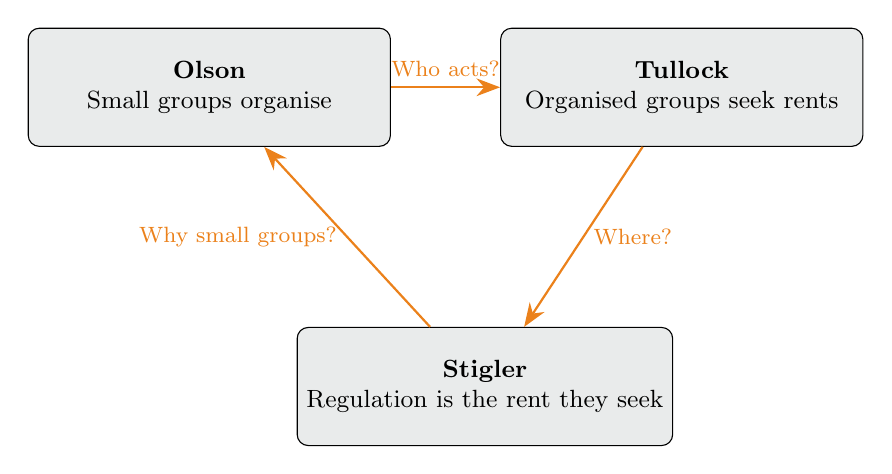
\begin{tikzpicture}[
box/.style={
draw,
rounded corners,
minimum width=4.6cm,
minimum height=1.5cm,
align=center,
font=\small,
fill=myTeal!10
},
arrow/.style={-{Stealth[length=3mm]}, thick, myOrange}
]


\node[box] (olson) at (-1,0)
{\textbf{Olson}\\Small groups organise};

\node[box] (tullock) at (5,0)
{\textbf{Tullock}\\Organised groups seek rents};

\node[box] (stigler) at (2.5,-3.8)
{\textbf{Stigler}\\Regulation is the rent they seek};


\draw[arrow] (olson) -- node[above, font=\footnotesize] {Who acts?} (tullock);
\draw[arrow] (tullock) -- node[right, font=\footnotesize] {Where?} (stigler);
\draw[arrow] (stigler) -- node[left, font=\footnotesize] {Why small groups?} (olson);

\end{tikzpicture}

\vspace{0.4cm}

\small
\textbf{Together:} Small groups organise (Olson), compete for rents (Tullock), 
and regulation is the mechanism through which those rents are obtained (Stigler).

Regulation creates rents → rents justify organisation → organisation sustains regulation.

\end{frame}

\begin{frame}{The Mirror Image: Why Good Policies Fail}
\textbf{The same logic works in reverse.}

\vspace{0.1cm}
Some policies generate \alert{concentrated costs} and \alert{dispersed benefits}:
\begin{itemize}
\item Trade liberalisation: benefits millions of consumers, but destroys the rents of a few protected firms
\item Planning reform: benefits future residents, but reduces current homeowners' property values
\item Professional deregulation: lowers prices for consumers, but cuts incumbents' incomes
\end{itemize}

\vspace{0.1cm}
\textbf{Olson's logic predicts:}
\begin{itemize}
\item The losers from reform are \emph{small, concentrated, and organised}
\item The winners are \emph{diffuse and often do not yet know they would benefit}
\item Result: welfare-improving reforms are systematically harder to enact
\end{itemize}

\vspace{0.1cm}
\alert{This is why protectionism is easier to introduce than to remove} - and why your opening steel tariff is more than a thought experiment.
\end{frame}

\begin{frame}{Final Thought}
\large

\begin{center}
Regulation is not only a response to market failure but also the outcome of political competition.
\end{center}


\begin{center}
When benefits are concentrated and costs are diffuse,
organised groups have an advantage.

That asymmetry shapes policy outcomes.

“If the members of a large group rationally seek to maximize their personal welfare, they will not act to achieve their common or group objective.”
— Olson (1965)
\end{center}

\end{frame}


\section*{Further Reading}

\begin{frame}{Foundations of Public Choice}
\footnotesize
\begin{enumerate}
\item Buchanan, J. \& Tullock, G. (1962). \emph{The Calculus of Consent}. University of Michigan Press.
\item Downs, A. (1957). \emph{An Economic Theory of Democracy}. Harper.
\item Olson, M. (1965). \emph{The Logic of Collective Action}. Harvard University Press.
\item Olson, M. (1982). \emph{The Rise and Decline of Nations}. Yale University Press.
\end{enumerate}
\end{frame}


\begin{frame}{Collective Action and Institutions}
\footnotesize
\begin{enumerate}
\item Hardin, R. (1982). \emph{Collective Action}. Johns Hopkins University Press.
\item Ostrom, E. (1990). \emph{Governing the Commons}. Cambridge University Press.
\end{enumerate}
\end{frame}

\begin{frame}{Rent-Seeking}
\footnotesize
\begin{enumerate}
\item Tullock, G. (1967). “The Welfare Costs of Tariffs, Monopolies, and Theft.” \emph{Western Economic Journal}.
\item Tullock, G. (1980). “Efficient Rent Seeking.” In Buchanan, Tollison \& Tullock (eds.), \emph{Toward a Theory of the Rent-Seeking Society}.
\item Krueger, A. (1974). “The Political Economy of the Rent-Seeking Society.” \emph{American Economic Review}.
\item Posner, R. (1975). “The Social Costs of Monopoly and Regulation.” \emph{Journal of Political Economy}.
\item Tollison, R. (1982). “Rent Seeking: A Survey.” \emph{Kyklos}.
\item Congleton, R., Hillman, A., \& Konrad, K. (Eds.) (2008). \emph{40 Years of Research on Rent Seeking}. Springer.
\end{enumerate}
\end{frame}

\begin{frame}{Regulation and Capture}
\footnotesize
\begin{enumerate}
\item Stigler, G. (1971). “The Theory of Economic Regulation.” \emph{Bell Journal of Economics}.
\item Peltzman, S. (1976). “Toward a More General Theory of Regulation.” \emph{Journal of Law and Economics}.
\item Becker, G. (1983). “A Theory of Competition Among Pressure Groups.” \emph{QJE}.
\item Dal B\'{o}, E. (2006). “Regulatory Capture: A Review.” \emph{Oxford Review of Economic Policy}.
\item Carpenter, D. \& Moss, D. (Eds.) (2013). \emph{Preventing Regulatory Capture}. Cambridge University Press.
\end{enumerate}
\end{frame}

\begin{frame}{Law, Institutions, and Regulation}
\footnotesize
\begin{enumerate}
\item Stewart, R. (1975). “The Reformation of American Administrative Law.” \emph{Harvard Law Review}.
\item Epstein, R. (1995). \emph{Simple Rules for a Complex World}. Harvard University Press.
\item Bork, R. (1978). \emph{The Antitrust Paradox}. Basic Books.
\item Yandle, B. (1983). “Bootleggers and Baptists.” \emph{Regulation}.
\item Smith, A. \& Yandle, B. (2014). \emph{Bootleggers and Baptists}. Cato Institute.
\item Carpenter, D. (2010). \emph{Reputation and Power}. Princeton University Press.
\end{enumerate}
\end{frame}

\begin{frame}{Irish Political Economy}
\footnotesize
\begin{enumerate}
\item Barrett, S. (2010). “Regulatory Capture, Property Rights and Taxi Deregulation.” \emph{Economic Affairs}.
\item Aisling, L. \& McLaughlin, E. (2022). Occupational Licensing in Ireland. ESRI Working Paper.
\item Lyons, R. (2021). \emph{The Rent Crisis}. Penguin Ireland.
\item MacCarthaigh, M. (2017). \emph{Public Sector Reform in Ireland}. IPA.
\end{enumerate}
\end{frame}


\section*{Cultural Resources}

\begin{frame}{Films \& Documentaries}
\textbf{Lobbying, Capture, and Special Interests:}
\begin{itemize}
\item \textbf{Thank You for Smoking} (2005) -- lobbying, framing, and the "Merchants of Doubt" strategy
\item \textbf{The Corporation} (2003) -- corporate influence on regulation
\item \textbf{Dark Waters} (2019) -- regulatory failure and corporate capture in chemical regulation
\item \textbf{Food, Inc.} (2008) -- agricultural lobbying and food regulation in the US
\end{itemize}
\end{frame}


\begin{frame}{TV Series}
\textbf{Politics, Lobbying, and Institutions:}
\begin{itemize}
\item \textbf{Yes Minister / Yes, Prime Minister} -- bureaucratic self-interest and regulatory inertia
\item \textbf{The Wire} (Season 2) -- unions, deindustrialisation, and rent-seeking
\item \textbf{Borgen} -- coalition politics, interest groups, and policy compromise
\item \textbf{Miss Sloane} (2016, film) -- inside a Washington lobbying firm
\end{itemize}
\end{frame}


\begin{frame}{Books for General Audience}
\begin{itemize}
\item Mancur Olson -- \emph{The Rise and Decline of Nations} (more accessible than \emph{Logic})
\item Luigi Zingales -- \emph{A Capitalism for the People}
\item Brink Lindsey \& Steven Teles -- \emph{The Captured Economy}
\end{itemize}
\end{frame}


\begin{frame}[allowframebreaks]{Podcasts \& Media}
\textbf{Political Economy:}
\begin{itemize}
\item \textbf{EconTalk} -- episodes on regulatory capture and rent-seeking
\item \textbf{Planet Money} -- episodes on occupational licensing ("So You Think You Can Be a Hair Braider")
\item \textbf{The Ezra Klein Show} -- episodes on housing policy and NIMBYism
\end{itemize}

\framebreak
\textbf{Data and Analysis:}
\begin{itemize}
\item \textbf{OpenSecrets.org} -- US lobbying expenditure data
\item \textbf{Transparency International Ireland} -- lobbying register data
\item \textbf{OECD iLibrary} -- comparative data on occupational licensing and regulation
\end{itemize}
\end{frame}



\appendix

\section*{Backup Slides}

\begin{frame}{Olson: Privileged and Latent Groups}
\textbf{Olson distinguishes three group types:}

\vspace{0.1cm}
\begin{itemize}
\item \textbf{Privileged group:} at least one member has enough at stake that they would provide the good \emph{alone}, even if others free-ride.

\item \textbf{Intermediate group:} no single member would act alone, but the group is small enough that each member's contribution is noticeable.

\item \textbf{Latent group:} so large that no individual's contribution matters.
Requires selective incentives or coercion to act.
\end{itemize}

\vspace{0.1cm}
\alert{Examples:}
A dominant firm lobbying for a tariff (privileged); a trade association of 20 firms (intermediate); all consumers of a product (latent).
\end{frame}


\begin{frame}{Tullock: Simple Rent-Seeking Model}
\textbf{A simplified contest:}

\vspace{0.1cm}
\begin{itemize}
\item A government-created rent of value $V$ is available
\item $N$ agents each choose expenditure $x_i$ to compete for it
\item Agent $i$'s probability of winning: $p_i = \frac{x_i}{\sum_j x_j}$
\item Agent $i$'s expected payoff: $p_i \cdot V - x_i$
\end{itemize}

\vspace{0.1cm}
\textbf{Nash equilibrium (symmetric):}
\[
x^* = \frac{(N-1)}{N^2} \cdot V
\]
\textbf{Total expenditure:}
\[
N \cdot x^* = \frac{(N-1)}{N} \cdot V
\]

\vspace{0.1cm}
\alert{As $N \to \infty$, total expenditure $\to V$:} the rent is fully dissipated.
\end{frame}


\begin{frame}{Stigler: Why Not Direct Subsidies?}
\textbf{If industries want money from the state, why not just ask for cash?}

\vspace{0.1cm}
Stigler argues that \alert{entry control is preferred} over direct subsidies for two reasons:

\vspace{0.1cm}
\begin{enumerate}
\item \textbf{Visibility:} direct cash transfers are politically salient and easy to oppose.
Entry restrictions are technical and opaque.

\vspace{0.1cm}
\item \textbf{Rent erosion:} a cash subsidy attracts new entrants who compete away the profit.
A licensing requirement \emph{prevents} new entry, so the rent persists.
\end{enumerate}

\vspace{0.1cm}
\alert{This explains a regularity:} the most durable forms of regulatory capture tend to involve entry barriers (licensing, permits, qualifications), not direct payments.
\end{frame}


\begin{frame}{Peltzman's Extension of Stigler}
\textbf{Peltzman (1976) formalised Stigler's insight:}

\vspace{0.1cm}
A regulator maximises political support by balancing:
\begin{itemize}
\item Support from the regulated industry (which wants higher prices)
\item Opposition from consumers (who want lower prices)
\end{itemize}

\vspace{0.1cm}
\textbf{The result:} the regulated price is set between the competitive and monopoly levels - not at the monopoly price, because that would provoke too much consumer opposition.

\vspace{0.1cm}
\alert{Implication:}
Regulation does not perfectly serve either group.
But it systematically favours the group that is better organised (Olson) and invests more in the political contest (Tullock).
\end{frame}


\begin{frame}{Counterarguments and Limitations}
\textbf{The Olson--Tullock--Stigler view is powerful but not complete:}

\vspace{0.1cm}
\begin{itemize}
\item \textbf{Successful large-group mobilisation does occur:}
environmental movements, civil rights, consumer protection.
Olson's theory may underpredict ideologically motivated action.

\vspace{0.1cm}
\item \textbf{Not all regulation is capture:}
some regulations genuinely correct market failures (safety standards, pollution limits).

\vspace{0.1cm}
\item \textbf{Institutions can constrain capture:}
transparency requirements, independent regulators, and sunset clauses can reduce (though not eliminate) capture.

\vspace{0.1cm}
\item \textbf{Becker (1983):}
competition among pressure groups may produce more efficient outcomes than Olson--Stigler suggests, because deadweight losses generate opposition.
\end{itemize}
\end{frame}


\begin{frame}{Bootleggers and Baptists: Irish Application}
\textbf{Ireland's Regulation of Lobbying Act (2015):}

\vspace{0.1cm}
\begin{itemize}
\item \textbf{Baptists:} transparency advocates and anti-corruption campaigners
\item \textbf{Potential bootleggers:} large, established lobbying firms that can easily comply with disclosure requirements
\end{itemize}

\vspace{0.1cm}
\textbf{The Yandle test:} does the regulation impose higher costs on small, informal advocacy groups than on professional lobbyists?
If so, the transparency framework may double as a barrier to entry in the "market" for political influence.

\vspace{0.1cm}
\alert{Irish climate policy} offers another example: large energy incumbents publicly support carbon targets while smaller competitors face disproportionate compliance burdens.
The "green" framing provides Baptist cover; the entry-barrier effect serves the bootlegger.
\end{frame}


\begin{frame}{The Revolving Door: Mechanisms and Evidence}
\textbf{Three channels through which the revolving door affects regulation:}

\vspace{0.1cm}
\begin{enumerate}
\item \textbf{Human capital (benign):}
Regulators hire from industry because that is where the expertise exists.
Can \emph{improve} regulatory quality.

\vspace{0.15cm}
\item \textbf{Incentive (problematic):}
A regulator who expects to join the industry afterwards has weakened incentives to enforce aggressively.

\vspace{0.15cm}
\item \textbf{Network (structural):}
Former colleagues on both sides share information informally, creating channels of influence that bypass formal processes.
\end{enumerate}

\vspace{0.1cm}
\alert{Dal B\'{o} (2006):} the revolving door is one of the most robust empirical correlates of regulatory outcomes favouring industry.
\end{frame}


\begin{frame}{Institutional Sclerosis: Testing Olson's Prediction}
\textbf{Olson's prediction generates testable hypotheses:}

\vspace{0.1cm}
\begin{itemize}
\item \textbf{Within countries:} US states with longer periods of stability should have more interest groups and slower growth (Olson finds support).
\item \textbf{Across countries:} defeated Axis powers (Germany, Japan) should outperform Britain, which retained its pre-war institutional structure.
\item \textbf{Post-crisis:} severe economic crises can "break" distributional coalitions, enabling previously blocked reforms.
\end{itemize}

\vspace{0.1cm}
\alert{Critiques:}
\begin{itemize}
\item Correlation between stability and interest groups doesn't prove causation
\item Post-war growth may reflect reconstruction, not sclerosis removal
\item Some long-stable democracies (Switzerland, Scandinavia) have strong interest groups \emph{and} high growth
\end{itemize}
\end{frame}


\begin{frame}{Concentrated Costs and Trade Liberalisation}
\textbf{Why is it so hard to remove protectionism?}

\vspace{0.1cm}
\begin{itemize}
\item A tariff removal that benefits 5m consumers by \euro 2 each but costs 5 firms \euro 2m each is a net welfare gain - but the \alert{political calculus} is asymmetric
\item The firms will lobby, litigate, and mobilise workers
\item Consumers will not even notice the price drop
\end{itemize}

\vspace{0.1cm}
\textbf{Policy design implication:}
Successful liberalisation often requires \alert{compensation} for the concentrated losers - not on efficiency grounds, but because without it the reform will never pass.

\vspace{0.1cm}
\alert{Examples:}
\begin{itemize}
\item EU structural funds as compensation for trade liberalisation
\item US Trade Adjustment Assistance for displaced workers
\item Dublin taxi plate compensation scheme after 2000 deregulation
\end{itemize}
\end{frame}


\end{document}